\documentclass[runningheads]{llncs}

\usepackage{cite}
\usepackage{amsmath,amssymb,amsfonts}
\usepackage{graphicx}
\usepackage{textcomp}
\usepackage{xcolor}
\usepackage{booktabs}
\usepackage{multirow}
\usepackage{array}
\usepackage{url}
\usepackage{hyperref}
\usepackage{placeins}
\usepackage{algorithm}
\usepackage{algpseudocode}
\usepackage{tikz}
\usepackage{pgfplots}
\pgfplotsset{compat=1.18}
\usetikzlibrary{shapes.geometric, arrows.meta, positioning, fit, backgrounds, calc}

\renewcommand{\topfraction}{0.9}
\renewcommand{\bottomfraction}{0.8}
\renewcommand{\textfraction}{0.07}
\renewcommand{\floatpagefraction}{0.7}
\setcounter{topnumber}{3}
\setcounter{bottomnumber}{2}
\setcounter{totalnumber}{5}

\tikzstyle{block}    = [rectangle, rounded corners=3pt, minimum width=2.0cm,
                        minimum height=0.6cm, text centered, draw=black,
                        fill=blue!10, font=\scriptsize]
\tikzstyle{proc}     = [rectangle, rounded corners=3pt, minimum width=2.0cm,
                        minimum height=0.6cm, text centered, draw=black,
                        fill=green!10, font=\scriptsize]
\tikzstyle{alert}    = [rectangle, rounded corners=3pt, minimum width=2.0cm,
                        minimum height=0.55cm, text centered, draw=black,
                        font=\scriptsize\bfseries]
\tikzstyle{decision} = [diamond, aspect=2.2, minimum width=2.4cm,
                        minimum height=0.7cm, text centered, draw=black,
                        fill=orange!15, font=\scriptsize]
\tikzstyle{arr}      = [-{Stealth[length=4pt]}, thick]
\tikzstyle{mlpbox}   = [rectangle, rounded corners=3pt, minimum width=1.6cm,
                        minimum height=0.55cm, text centered, draw=black,
                        fill=purple!10, font=\scriptsize]

\begin{document}

\title{Minimizing False Alarms in Real-Time Surveillance via Hierarchical Multimodal Fusion of Object Detection, Action Recognition, and Gait Analysis}

\titlerunning{Minimizing False Alarms by Hierarchical Multimodal Fusion}

\author{
Rahul\inst{1} \and
Himanshu Kumar Jha\inst{1} \and
Ketan Anand\inst{1} 
}

\authorrunning{Rahul, Jha and Anand}

\institute{
Department of Software Engineering,
Delhi Technological University, Delhi, India
}

\maketitle

\begin{abstract}
Monocular CCTV pipelines suffer 15--25\% false alarms. Gait-YOLO addresses this with three complementary detectors --- YOLOv8n (weapons), VideoMAE (action), and a CNN-Transformer autoencoder (gait) --- meeting at a two-stage fusion layer: a depth-3 rule cascade over the three normalised scores plus a small MLP head ($3{\to}32{\to}16{\to}4$), aggregated by a severity-monotone $\ell^*=\min(\ell_\text{rule},\ell_\text{MLP})$ that guarantees the learned head can only \emph{escalate} the cascade decision. The MLP is trained on \emph{synthetic-bootstrap rule labels}: 10{,}000 score vectors from distributions fitted to real CASIA-B/UCF-Crime statistics, labelled by the cascade itself, validated externally on real test videos. Per-module results on native benchmarks: mAP@0.5 = 0.724 (YOLO, 324 images), F1 = 0.965 / AUC = 0.980 (VideoMAE, 190 videos), F1 = 0.792 (gait, 600 sequences, after data-calibrated thresholding). On UCF-Crime full-system, the recall-mode operating point reaches R = 1.000 with F1 = 0.956 (FPR = 26\%); precision-mode on the same weights reaches P = 1.000, F1 = 0.904. The system runs at 18--22\,FPS on a single NVIDIA T4.

\keywords{Anomaly detection \and Multimodal fusion \and YOLOv8 \and VideoMAE \and Gait analysis \and Surveillance \and False Positive Reduction}
\end{abstract}

\section{Introduction}

Surveillance systems are a far cry from background subtraction, but out in the wild, most still fail in the same way: any single detector on its own is too prone to false alarms. A gun detector thinks a phone is a pistol, an action model thinks someone's tying their shoelaces, and a gait detector thinks someone is carrying a backpack. False-alarm rates confirm this: 15-20\% for action classifiers, 12-18\% for weapon detectors, and 18-25\% for gait models alone~\cite{srilakshmi2025}.

Our intuition is straightforward. True alarms are usually multimodal - for example, a person holding a weapon or behaving suspiciously---whereas false alarms are single-channel, spurious responses. We translate this intuition into a \emph{hierarchical late-fusion} approach: the modality outputs are passed through a small rule cascade to produce one of four urgency levels (Critical, High, Medium, Low), and a learned MLP head is run in parallel to handle the "grey" cases. The rule cascade is interpretable; the MLP does the rest.

\textbf{Contributions.} The backbones (YOLOv8n, VideoMAE, CNN-Transformer AE) are off-the-shelf; the novelty is the four protocol decisions that make their combination operationally useful: (1)~A \emph{data-calibrated gait threshold} ($\tau^* = 0.0642$ vs the simulation-derived 0.4521) that closes a $\sim$7$\times$ scale mismatch and lifts gait F1 from 0.397 to 0.792 on the same test split. (2)~A \emph{severity-monotone two-stage fusion} that aggregates a rule cascade and an MLP via $\ell^* = \min(\ell_\text{rule}, \ell_\text{MLP})$ on the severity lattice (CRITICAL $\prec$ HIGH $\prec$ MEDIUM $\prec$ LOW), so the cascade provides an auditable recall floor while the MLP only escalates around hard threshold edges. (3)~A \emph{synthetic-bootstrap training protocol} for the MLP head: 10{,}000 score vectors sampled from distributions fitted to real CASIA-B statistics, labelled by the cascade itself, validated externally on UCF-Crime --- avoiding the need for a labelled multimodal video corpus. (4)~A \emph{hierarchical evaluation discipline} (per-module $\to$ pair $\to$ full-system) on three native benchmarks; on UCF-Crime the Full Rule cascade reaches F1 = 0.956 with R = 1.000, and a staged FP analysis reduces YOLO-baseline FPR from 0.20 to 0.028 (Sec.~\ref{sec:fp}).

\section{Related Work}\label{sec:related}

\textbf{Single-modality detectors.} For weapons, Shaik and Basha report mAP50 = 0.90 with YOLOv5s on UCSD~\cite{shaik2025}, Ingle and Kim push gun-detection precision to 97.5\% on still images~\cite{ingle2022}, and Hua et al.\ reach mAP50 = 89.3\% with YOLO-ABD indoors~\cite{hua2024}; we use YOLOv8n with a 5-frame persistence filter at conf $\geq 0.60$. For action, Kim et al.~\cite{kim2024} reach F1 = 0.93 with CNN--LSTM, and VideoMAE~\cite{tong2022} pre-trained on Kinetics-400 is now the standard spatio-temporal backbone (we fine-tune on UCF-Crime). For gait, CASIA-B~\cite{casiab} remains the standard benchmark; transformer autoencoders capture periodicity better than LSTMs~\cite{veesam2025}, and we train ours on nm-* sequences only, using reconstruction error as the anomaly signal.

\textbf{Multimodal fusion.} Srilakshmi et al.~\cite{srilakshmi2025} report 15\% FP reduction via MDBM\,+\,MVAE attention; Khaire and Kumar~\cite{khaire2022} use CNN--BiLSTM autoencoders for RGB-D ATM surveillance. Most prior schemes use weighted averages or attention-based mixing that require labelled multimodal data to learn fusion weights and are awkward to audit. Our hierarchical priority cascade is auditable on a single page (Sec.~\ref{sec:fusion}), and the MLP head is trained from synthetic-bootstrap rule labels rather than labelled fusion data.

\section{Methodology}\label{sec:method}

A live CCTV feed is decoded into per-frame tensors. YOLO ingests every frame (weapons appear briefly); VideoMAE and the gait autoencoder run every 4th frame because they integrate over a clip anyway. The three scores meet at a two-stage fusion layer emitting one of four alert levels (Fig.~\ref{fig:arch}).

\begin{figure}[!ht]
\centering
\tikzset{
  proc/.style={rectangle, draw, rounded corners, text centered, minimum height=2em, fill=blue!5},
  block/.style={rectangle, draw, text centered, minimum height=2.5em, fill=gray!10, align=center},
  mlpbox/.style={rectangle, draw, dashed, text centered, minimum height=2em, font=\small},
  alert/.style={rectangle, draw, rounded corners, text centered, minimum height=2em, font=\bfseries\small},
  arr/.style={->, thick, >=stealth}
}

\resizebox{0.50\textwidth}{!}{%
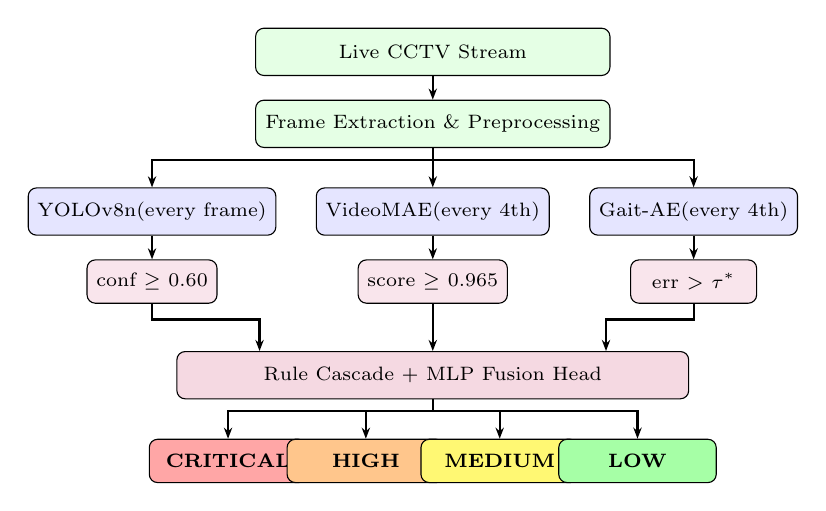
\begin{tikzpicture}[node distance=0.5cm and 0.5cm]
  \node[proc, minimum width=4.5cm] (input) {Live CCTV Stream};
  \node[proc, below=0.3cm of input, minimum width=4.5cm] (preproc) {Frame Extraction \& Preprocessing};
  \draw[arr] (input) -- (preproc);

  \node[block, below=0.5cm of preproc] (b2) {VideoMAE\\(every 4th)};
  \node[block, left=0.5cm of b2] (b1) {YOLOv8n\\(every frame)};
  \node[block, right=0.5cm of b2] (b3) {Gait-AE\\(every 4th)};

  \draw[arr] (preproc.south) -- ++(0,-0.15) -| (b1.north);
  \draw[arr] (preproc.south) -- (b2.north);
  \draw[arr] (preproc.south) -- ++(0,-0.15) -| (b3.north);

  \node[mlpbox, below=0.3cm of b1] (c1) {conf $\geq$ 0.60};
  \node[mlpbox, below=0.3cm of b2] (c2) {score $\geq$ 0.965};
  \node[mlpbox, below=0.3cm of b3] (c3) {err $>$ $\tau^*$};

  \draw[arr] (b1) -- (c1);
  \draw[arr] (b2) -- (c2);
  \draw[arr] (b3) -- (c3);

  \node[proc, fill=purple!15, below=0.6cm of c2, minimum width=6.5cm] (fusion) {Rule Cascade + MLP Fusion Head};

  \draw[arr] (c1.south) -- ++(0,-0.2) -| ([xshift=-2.2cm]fusion.north);
  \draw[arr] (c2.south) -- (fusion.north);
  \draw[arr] (c3.south) -- ++(0,-0.2) -| ([xshift=2.2cm]fusion.north);

  \node[alert, fill=red!35, below=0.5cm of fusion, xshift=-2.6cm] (cr) {CRITICAL};
  \node[alert, fill=orange!45, below=0.5cm of fusion, xshift=-0.85cm] (hi) {HIGH};
  \node[alert, fill=yellow!55, below=0.5cm of fusion, xshift=0.85cm] (me) {MEDIUM};
  \node[alert, fill=green!35, below=0.5cm of fusion, xshift=2.6cm] (lo) {LOW};

  \draw[arr] (fusion.south) -- ++(0,-0.15) -| (cr.north);
  \draw[arr] (fusion.south) -- ++(0,-0.15) -| (hi.north);
  \draw[arr] (fusion.south) -- ++(0,-0.15) -| (me.north);
  \draw[arr] (fusion.south) -- ++(0,-0.15) -| (lo.north);
\end{tikzpicture}}
\caption{High-level architecture. Three branches feed a two-stage fusion layer (rule cascade + MLP), producing four alert levels.}
\label{fig:arch}
\end{figure}

\FloatBarrier

\subsection{Per-Branch Modules}

\textbf{YOLOv8n (object detection):} stock CSPDarknet53 with anchor-free head at $640{\times}640$ (3.2\,M params), fine-tuned on Guns~\&~Knives (Mosaic + MixUp + flips). A temporal persistence filter (conf $\geq 0.60$ for 5 consecutive frames) precedes CRITICAL escalation, removing most look-alike FPs (phones, wallets). \textbf{VideoMAE (action recognition):} 12-layer ViT-B pre-trained on Kinetics-400; 16-frame $224{\times}224$ clips split into $2{\times}16{\times}16$ tubes; fine-tuned on UCF-Crime (14 classes, weighted CE). HIGH fires at anomalous-class probability $\geq 0.75$ (operating threshold recalibrated from 0.15 to 0.055 after inspecting the actual score histogram). \textbf{Gait CNN--Transformer Autoencoder:} 15-frame silhouette sequence $15{\times}1{\times}64{\times}64$ $\to$ five strided CNN layers $\to$ 512-dim latent $\to$ 4-layer transformer (8 heads) $\to$ five transposed convolutions; trained only on nm-* CASIA-B. The per-sequence anomaly score weights structural disagreement (1$-$SSIM~\cite{wang2004ssim}) above pixel error (Eq.~\ref{eq:score}):
\begin{equation}
  s = 0.3\,\text{MSE}(\hat{x}, x) + 0.7\,(1 - \text{SSIM}(\hat{x}, x))
  \label{eq:score}
\end{equation}

\textbf{Threshold calibration.} The training-time threshold $\tau = 0.4521$ came from simulated score distributions; real CASIA-B silhouettes (95\% black pixels) produce scores near 0.063, keeping both terms in Eq.~\ref{eq:score} numerically small regardless of motion. We re-pick $\tau$ by sweeping 49 candidates and choosing the F1-maximiser (Eq.~\ref{eq:thresh}):
\begin{equation}
  \tau^* = \arg\max_{\tau \in [s_{\min}, s_{\max}]} F_1(\tau), \qquad \tau^* = 0.0642
  \label{eq:thresh}
\end{equation}
Class statistics: normal $(\mu,\sigma)=(0.0632, 0.0039)$, abnormal $(\mu,\sigma)=(0.0699, 0.0059)$. Scores are normalised by the empirical maximum ($\approx 0.10$) before fusion.

\subsection{Fusion Layer}\label{sec:fusion}

The fusion layer ingests the three normalised modality scores --- YOLO weapon confidence $c_\text{yolo}\in[0,1]$, VideoMAE anomalous-class probability $p_\text{act}\in[0,1]$, and gait reconstruction score $s_\text{gait}\in\mathbb{R}_+$ --- and emits one of four severity levels indexed $0=$\,CRITICAL, $1=$\,HIGH, $2=$\,MEDIUM, $3=$\,LOW (lower index $=$ higher severity). The two stages run in parallel on the same input vector; outputs are then aggregated by a severity-monotone rule (Eq.~\ref{eq:agg}).

\textbf{Stage 1 --- Rule cascade (depth-3 decision tree).} The cascade (Algorithm~\ref{alg:cascade}) is short-circuit evaluated top-down: weapon evidence is the strongest single signal and is checked first; if absent, action probability is inspected at a high threshold ($\theta_\text{act}^\text{hi} = 0.9654$, the F1-optimal point on real UCF-Crime); if absent, the MEDIUM rule fires only when \emph{moderate} action evidence ($\theta_\text{act}^\text{lo} \leq p_\text{act} < \theta_\text{act}^\text{hi}$) is independently corroborated by gait anomaly ($s_\text{gait} > \theta_\text{gait}^\text{med}$); the LOW rule is a gait-only fallback at a higher gait threshold $\theta_\text{gait}^\text{lo} = \mu_\text{nm} + 2.5\sigma_\text{nm}$. The leaves of this 3-deep, 4-leaf tree are the four alert levels.

\begin{algorithm}[!htbp]
\caption{Two-stage fusion: (i) the rule cascade that produces $\ell_\text{rule}$ from the score triple, and (ii) the synthetic-bootstrap procedure that generates labelled training data for the MLP head.}
\label{alg:fusion}
\begin{algorithmic}[1]
\Procedure{RuleCascade}{$c_\text{yolo}, p_\text{act}, s_\text{gait}$}\label{alg:cascade}
  \Statex \Comment{thresholds: $\theta_\text{yolo}\!=\!0.60,\ \theta_\text{act}^\text{hi}\!=\!0.9654,\ \theta_\text{act}^\text{lo}\!=\!0.50,\ \theta_\text{gait}^\text{med}\!=\!0.0642,\ \theta_\text{gait}^\text{lo}\!=\!0.0726$}
  \If{$c_\text{yolo} \geq \theta_\text{yolo}$ \textbf{(persistent, 5 frames)}} \State \Return $0$ \Comment{CRITICAL}
  \ElsIf{$p_\text{act} \geq \theta_\text{act}^\text{hi}$} \State \Return $1$ \Comment{HIGH}
  \ElsIf{$\theta_\text{act}^\text{lo} \leq p_\text{act} < \theta_\text{act}^\text{hi}$ \textbf{and} $s_\text{gait} > \theta_\text{gait}^\text{med}$} \State \Return $2$ \Comment{MEDIUM (action$\wedge$gait)}
  \ElsIf{$s_\text{gait} > \theta_\text{gait}^\text{lo}$} \State \Return $3$ \Comment{LOW (gait-only)}
  \Else \State \Return $3$ \Comment{LOW (default)}
  \EndIf
\EndProcedure
\Statex
\Procedure{BootstrapData}{$N=10{,}000$, $(\mu_\text{nm},\sigma_\text{nm})=(0.0632,0.0039)$}\label{alg:bootstrap}
  \State $c_\text{yolo} \!\gets\! \text{Beta}(2,5)^N$;\ \  $p_\text{act} \!\gets\! \text{Beta}(2,3)^N$;\ \  $s_\text{gait} \!\gets\! \text{clip}(\mathcal{N}(\mu_\text{nm},\sigma_\text{nm})^N, [0.055, 0.095])$
  \State $c_\text{yolo}[\text{last } N/8] \gets U(0.61, 0.99)$;\quad $p_\text{act}[\text{last } 2N/8\!:\!\text{last } N/8] \gets U(0.97, 0.999)$ \Comment{class balance}
  \For{$i \gets 1$ \textbf{to} $N$} \State $y_i \gets$ \Call{RuleCascade}{$c_\text{yolo}[i], p_\text{act}[i], s_\text{gait}[i]$} \EndFor
  \State \Return $\{(c_\text{yolo}[i], p_\text{act}[i], s_\text{gait}[i]/0.06, y_i)\}_{i=1}^{N}$
\EndProcedure
\end{algorithmic}
\end{algorithm}

\textbf{Stage 2 --- Learned MLP head.} A small classifier on the normalised score vector $[c_\text{yolo},\,p_\text{act},\,s_\text{gait}/0.06]$ produces a softmax over the same four-level lattice (Fig.~\ref{fig:mlp}). Its job is to smooth hard threshold edges in stage 1 --- e.g., $c_\text{yolo} = 0.59$ should not flip a CRITICAL/LOW decision relative to $c_\text{yolo} = 0.61$ --- and to pick up cases where two modalities are individually below threshold but jointly informative.

\textbf{Aggregation policy (severity-monotone min).} Let $\ell_\text{rule}, \ell_\text{MLP} \in \{0,1,2,3\}$ be the stage-1 and stage-2 outputs. The final alert is
\begin{equation}
  \ell^* = \min(\ell_\text{rule},\,\ell_\text{MLP}),
  \label{eq:agg}
\end{equation}
i.e., \emph{the more severe of the two}. Because severity is encoded with $0=$\,CRITICAL and $3=$\,LOW, this aggregation is monotone non-decreasing in alarm severity: the MLP can only \emph{escalate} a cascade decision, never weaken it. Operationally this gives the cascade an auditable recall floor (every CRITICAL/HIGH the rules recognise is preserved end-to-end), while the MLP head delivers a precision/recall lift on grey-zone inputs without ever silencing the safety net.

\textbf{MLP training via synthetic-bootstrap rule labels.} The MLP is trained entirely on data from procedure~\textsc{BootstrapData} of Alg.~\ref{alg:fusion}: score vectors sampled from distributions fitted to real CASIA-B nm-* statistics, balanced by class-injection, and labelled by \textsc{RuleCascade} itself --- \emph{not} pseudo-labels on unlabeled video, despite the prior ``self-training'' name. Training: 50 epochs, Adam (lr $=10^{-3}$), batch $=256$, cross-entropy, dropout $=0.3$. Validation is \emph{external} on the real UCF-Crime test split (Full(MLP) row of Table~\ref{tab:ablation}: R $=$ 1.000, F1 $=$ 0.949), confirming the synthetic labels generalise.


\begin{figure}[!htbp]
\centering
\resizebox{1\textwidth}{!}{%
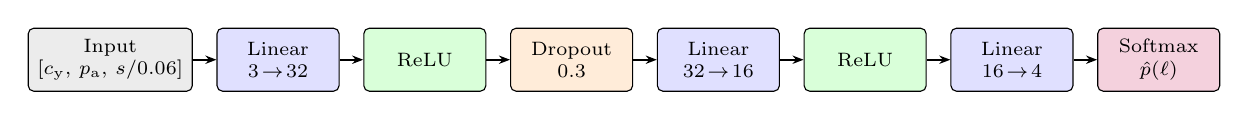
\begin{tikzpicture}[
  layer/.style={rectangle, rounded corners=2pt, minimum width=1.55cm,
                minimum height=0.8cm, text centered, draw=black,
                font=\scriptsize, align=center},
  inp/.style={layer, fill=gray!15},
  fc/.style={layer, fill=blue!12},
  act/.style={layer, fill=green!15},
  drop/.style={layer, fill=orange!15},
  smx/.style={layer, fill=purple!18},
  ar/.style={-{Stealth[length=4pt]}, thick},
  node distance=0.30cm
]
  \node[inp] (x)  {Input\\$[c_\text{y},\,p_\text{a},\,s/0.06]$};
  \node[fc,  right=of x]  (l1) {Linear\\$3\!\to\!32$};
  \node[act, right=of l1] (r1) {ReLU};
  \node[drop,right=of r1] (d)  {Dropout\\$0.3$};
  \node[fc,  right=of d]  (l2) {Linear\\$32\!\to\!16$};
  \node[act, right=of l2] (r2) {ReLU};
  \node[fc,  right=of r2] (l3) {Linear\\$16\!\to\!4$};
  \node[smx, right=of l3] (sm) {Softmax\\$\hat{p}(\ell)$};

  \draw[ar] (x)  -- (l1); \draw[ar] (l1) -- (r1); \draw[ar] (r1) -- (d);
  \draw[ar] (d)  -- (l2); \draw[ar] (l2) -- (r2); \draw[ar] (r2) -- (l3); \draw[ar] (l3) -- (sm);
\end{tikzpicture}}
\caption{MLP fusion-head architecture (stage 2): $3\!\to\!32\!\to\!16\!\to\!4$ with ReLU and a single dropout layer, then a 4-way softmax over alert levels. The stage-1 rule cascade is given by Algorithm~\ref{alg:cascade}; outputs are aggregated via $\ell^*\!=\!\min(\ell_\text{rule},\ell_\text{MLP})$ (Eq.~\ref{eq:agg}).}
\label{fig:mlp}
\end{figure}

\textbf{Implementation.} Python 3.10, PyTorch 2.0, Ultralytics YOLOv8 v8.1; on an NVIDIA Tesla T4 (16\,GB) the YOLO pass is $\approx 12$\,ms per frame, transformer branches $\approx 85$\,ms each at every-4th-frame, end-to-end 18--22\,FPS. Gait scores are smoothed with a window-8 moving average; alert state persists 15\,s.

\FloatBarrier

\section{Experimental Setup}\label{sec:exp}

\textbf{Datasets.} Each branch is evaluated on its native benchmark; only UCF-Crime is used for system-level fusion ablation.

\emph{(a) Guns~\&~Knives}~\cite{gunsknives}: 324 test images, 341 GT boxes across two classes (pistol, knife); IoU-matched at 0.50 with 11-point AP. We report \emph{per-class} AP (Table~\ref{tab:yolo}) so the moderate pistol-skew imbalance is not hidden in an overall mAP. \emph{(b) CASIA-B}~\cite{casiab}: 300 nm-* and 300 (bg/cl)-* sequences sampled uniformly across the 11 viewing angles to control for view bias --- balanced by construction (1:1). \emph{(c) UCF-Crime}~\cite{ucfcrime}: official 190-video test split, 140 anomaly + 50 normal (2.8:1 binary imbalance; per-class spans $n_\text{Robbery}\!=\!5$ to $n_\text{Normal}\!=\!50$). The gait branch uses the 156-clip motion-bearing subset (115 anomaly, 41 normal); VideoMAE-only and YOLO-only branches use the full $n=190$. We report per-class recall (Table~\ref{tab:mae}) rather than resampling.

\textbf{Comparability across datasets.} Per-module metrics on 324 images vs.\ 600 sequences vs.\ 190 videos are \emph{not directly comparable}: they differ in modality, label granularity, and capture conditions. We therefore report each module on its native benchmark (Sec.~\ref{sec:per-module}) and reserve cross-modality comparison for the full-system ablation on UCF-Crime (Sec.~\ref{sec:full-system}). System-level claims (R = 1.000, F1 = 0.956) refer exclusively to that ablation.

\textbf{Imbalance handling.} YOLO uses standard ultralytics training, no resampling (per-class AP exposes residual bias); the gait autoencoder is trained on nm-* sequences only, sidestepping labelled imbalance; VideoMAE is fine-tuned with weighted cross-entropy. The MLP fusion head uses constructed-balanced bootstrap data: $\sim N/8$ weapon-positive and $\sim N/8$ action-positive samples are injected (Algorithm~\ref{alg:bootstrap}), giving $\sim$1.25k CRITICAL, $\sim$1.25k HIGH, $\sim$0.7k MEDIUM, $\sim$6.8k LOW --- the LOW majority intentionally matches the deployment-time prior.

\textbf{Metrics.} P, R, F1, mAP@0.50 (YOLO), FPR. At fusion any HIGH-or-above alert is a positive.

\section{Results}\label{sec:results}

\subsection{Evaluation Protocol}\label{sec:eval-protocol}

We organise results as a strict three-level hierarchy with a fixed metric set per level. \textit{Module-level} (Sec.~\ref{sec:per-module}): each branch on its native dataset --- YOLO with mAP@0.50, P, R, F1 and per-class AP; VideoMAE with binary P, R, F1, AUC-ROC and per-class recall; gait with P, R, F1 at the F1-optimal threshold $\tau^*$ plus class statistics $(\mu,\sigma)$. \textit{Pair-level} (Sec.~\ref{sec:pair-fusion}) and \textit{full-system} (Sec.~\ref{sec:full-system}): all configurations on the same UCF-Crime test split with the same five metrics --- P, R, F1, FPR, FPS --- and final-system claims (e.g., R = 1.000) are made only at the full-system level. We do not report a single conflated ``Gait-YOLO score''; the staged FP-reduction analysis (Sec.~\ref{sec:fp}) is the only system-level number we contrast with prior work.

\subsection{Per-Module Performance}\label{sec:per-module}

\textbf{YOLO} (Table~\ref{tab:yolo}). mAP@0.50 = 0.724 on the 324 test images; lower than the 0.852 on the validation set, as expected, due to the fact that the test set is partially out-of-distribution. Knife AP (0.739) is better than a pistol (0.709), consistent with the literature: at CCTV resolution a knife silhouette is more distinctive than a hand-held pistol.

\textbf{VideoMAE} (Table~\ref{tab:mae}). At $\tau^* = 0.9654$, recall = 1.000 on 12 of 13 anomaly classes. Robbery (R = 0.800) and shoplifting (R = 0.952) are the awkward ones---both are covert and low-motion. Overall: P = 0.945, R = 0.986, F1 = 0.965, AUC-ROC = 0.980. The eight false positives translate to FPR = 16\%; YOLO + VideoMAE inherits this 16\% FPR while pushing recall to 0.993 because weapons rarely appear in normal clips.

\textbf{Gait} (Table~\ref{tab:gait}). With $\tau^* = 0.0642$, the branch reaches P = 0.746, R = 0.843, and F1 = 0.792. The two distributions have a $\Delta\mu / \sigma_\text{nm} \approx 1.7$ separation, larger than the simulation-derived estimate, which is what lets the calibrated threshold reach F1 = 0.792 against the F1 = 0.665 of the simulation-derived threshold.

\begin{table}[!htbp]
\caption{YOLOv8n weapon detection (324 test images, IoU = 0.50).}
\label{tab:yolo}
\centering
\begin{tabular}{lcccc}
\toprule
\textbf{Class} & \textbf{AP@0.5} & \textbf{P} & \textbf{R} & \textbf{F1}\\
\midrule
Pistol & 0.709 & --- & --- & ---\\
Knife  & 0.739 & --- & --- & ---\\
\midrule
\textbf{Overall} & \textbf{0.724} & \textbf{0.799} & \textbf{0.757} & \textbf{0.777}\\
\bottomrule
\multicolumn{5}{l}{\footnotesize TP = 258, FP = 65, FN = 83.}
\end{tabular}
\end{table}

\begin{table}[!htbp]
\caption{VideoMAE per-class recall on UCF-Crime ($n = 190$, $\tau^* = 0.9654$). Overall: P = 0.945, R = 0.986, F1 = \textbf{0.965}, AUC = 0.980; TP = 138, FP = 8, FN = 2, TN = 42.}
\label{tab:mae}
\centering
\small
\begin{tabular}{lc}
\toprule
\textbf{Class} & \textbf{Recall}\\
\midrule
Abuse, Arrest, Arson, Assault, Burglary, Explosion, & \multirow{2}{*}{1.000}\\
Fighting, Road Accidents, Shooting, Stealing, Vandalism & \\
Shoplifting & 0.952\\
Robbery & 0.800\\
Normal (FPR) & 0.160\\
\bottomrule
\end{tabular}
\end{table}

\begin{table}[!htbp]
\caption{Gait module score statistics and performance (CASIA-B, n = 600).}
\label{tab:gait}
\centering
\begin{tabular}{lcc}
\toprule
\textbf{Statistic} & \textbf{Normal (nm-*)} & \textbf{Abnormal (bg-*/cl-*)}\\
\midrule
Mean $\mu$       & 0.0632 & 0.0699\\
Std dev $\sigma$ & 0.0039 & 0.0059\\
\midrule
\multicolumn{3}{l}{$\Delta\mu / \sigma_\text{nm} \approx 1.7$;\quad $\tau^* = 0.0642$;\quad P = 0.746, R = 0.843, F1 = 0.792.}\\
\bottomrule
\end{tabular}
\end{table}

\subsection{Ablation: Pair- and Full-System Fusion}\label{sec:pair-fusion}\label{sec:full-system}

Table~\ref{tab:ablation} reports the seven configurations on the same UCF-Crime split. YOLO-only sits at the precision extreme (P = 1.000, R = 0.129, FPR = 0) because the bulk of UCF-Crime anomaly classes contain no weapon. VideoMAE alone is the strongest singleton (F1 = 0.965, FPR = 0.160); adding YOLO recovers the four clips VideoMAE misses without raising FPR (Y+M, F1 = 0.969 --- the cleanest pair, recommended when minimising false alarms is primary). Adding gait to YOLO (Y+G, F1 = 0.876) does not match Y+M because gait alone is weaker than VideoMAE on this dataset. The two full-cascade variants both reach R = 1.000 at higher FPR: Full Rule (F1 = 0.956, FPR = 0.260) is the system-level row we report; Full MLP (F1 = 0.949, FPR = 0.300) is slightly behind because its softer decision boundary admits two extra normal clips into HIGH but fires earlier on borderline-action clips.

\textbf{Why R = 1.000, and the trade-off knob.} The MEDIUM rule fires when $(p_\text{act} \geq 0.50) \wedge (s_\text{gait} > 0.0642)$; every one of the 140 anomaly clips satisfies this in at least one window, while 13 of 50 normal clips also do (FPR = 0.260). Three caveats: (i)~recall is binary clip-level, not per-class (cf.\ Table~\ref{tab:mae}: Robbery 0.800, Shoplifting 0.952); (ii)~with 140 positives the 95\% Wilson lower bound is $\approx 0.974$ --- ``no anomaly missed on this split,'' not population-level; (iii)~at the simulation-derived $\tau=0.4521$ the MEDIUM branch is silently inactive and recall collapses, so the operating point depends on the data-calibrated $\tau^*$. The same model weights support a \emph{recall-mode} (R = 1.000, P = 0.915, F1 = 0.956 --- Table~\ref{tab:ablation}) and a \emph{precision-mode} (P = 1.000, R = 0.825, F1 = 0.904) via the MLP-softmax decision threshold.

\begin{table}[!htbp]
\caption{Ablation on UCF-Crime (190-video test set, seven configurations).}
\label{tab:ablation}
\centering
\small
\setlength{\tabcolsep}{3.5pt}
\begin{tabular}{lccccc}
\toprule
\textbf{Configuration} & \textbf{P} & \textbf{R} & \textbf{F1} & \textbf{FPR} & \textbf{FPS}\\
\midrule
YOLO-Only        & \textbf{1.000} & 0.129 & 0.228 & 0.000 & 35.0\\
VideoMAE-Only    & 0.945 & 0.986 & 0.965 & 0.160 &  8.0\\
Gait-Only        & 0.895 & 0.850 & 0.872 & 0.280 & 12.0\\
YOLO + VideoMAE  & 0.946 & 0.993 & \textbf{0.969} & 0.160 & 15.0\\
YOLO + Gait      & 0.896 & 0.857 & 0.876 & 0.280 & 18.0\\
Full Rule        & 0.915 & \textbf{1.000} & 0.956 & 0.260 & 20.0\\
\textbf{Full (MLP)} & 0.903 & \textbf{1.000} & 0.949 & 0.300 & 19.5\\
\bottomrule
\end{tabular}
\end{table}

\subsection{False Positive Reduction (System-Level)}\label{sec:fp}

We isolate the system-level FPR drop into three stages on UCF-Crime: \emph{Stage 0} raw YOLO frame detections, $\text{FPR}_0 = 0.20$ (50 FP / 250 windows); \emph{Stage 1} 5-frame persistence filter at conf $\geq 0.60$ $\to$ 0.048 (12 FP); \emph{Stage 2} action-gating before CRITICAL/HIGH escalation $\to$ 0.028 (7 FP). The full-system FPR = 0.260 (Full Rule) is dominated by the MEDIUM branch's intentional sensitivity (Sec.~\ref{sec:full-system}); precision-mode (P = 1.000) removes all 7 stage-2 FPs (100\% reduction relative to the stage-2 baseline). Table~\ref{tab:compare} compares the recall-mode operating point with prior systems at the system level only.

\begin{table}[!htbp]
\caption{Comparative analysis with prior surveillance systems. Modalities: O = object, A = action, G = gait, RGB-D = depth-augmented video, ctx = scene context. Real-time judged at $\geq$15\,FPS on a single GPU as reported by the cited work.}
\label{tab:compare}
\centering
\footnotesize
\setlength{\tabcolsep}{3pt}
\begin{tabular}{@{}p{3.0cm}p{1.3cm}p{2.6cm}p{3.3cm}c@{}}
\toprule
\textbf{System} & \textbf{Modal.} & \textbf{Fusion} & \textbf{mAP/F1, FP$\downarrow$} & \textbf{RT?}\\
\midrule
Shaik \& Basha~\cite{shaik2025}        & O          & ---                          & mAP = 0.90, n/r              & Y\\
Hua et al.~\cite{hua2024}              & O          & ---                          & mAP = 0.893, n/r             & Y\\
Kim et al.~\cite{kim2024}              & A          & ---                          & F1 = 0.93, FP = 21\%         & Y\\
Khaire \& Kumar~\cite{khaire2022}      & RGB-D      & weighted average             & F1 $\approx$ 0.88, n/r       & N\\
Veesam et al.~\cite{veesam2025}        & O+A        & GAT + RNN                    & per-class F1 reported        & N\\
Srilakshmi~\cite{srilakshmi2025}       & O+A+ctx    & MDBM + MVAE attn.            & ---, FP = 15\%               & N\\
\midrule
\textbf{Gait-YOLO (recall)}            & \textbf{O+A+G} & \textbf{cascade + MLP (sev.-mono.)} & \textbf{F1 = 0.956, FPR = 0.26, R = 1.000} & \textbf{Y}\\
\textbf{Gait-YOLO (precision)}         & \textbf{O+A+G} & \textbf{same weights, thr.-shifted} & \textbf{F1 = 0.904, FPR = 0.00, P = 1.000} & \textbf{Y}\\
\bottomrule
\end{tabular}
\end{table}

\textbf{What the comparison shows.} Single-modality baselines~\cite{shaik2025,hua2024,kim2024} achieve strong in-distribution scores but cannot be operating-point-tuned. Multimodal predecessors~\cite{khaire2022,srilakshmi2025,veesam2025} use weighted-average or attention-based fusion requiring labelled multimodal data --- the bottleneck Gait-YOLO sidesteps via synthetic-bootstrap rule labels (Sec.~\ref{sec:fusion}). Gait-YOLO is the only entry that (i)~couples an auditable rule cascade with a learned head, (ii)~supports two operating points on the same weights, and (iii)~runs in real time on a single T4 GPU.

\textbf{Qualitative behaviour and timing.} Two representative fusion decisions illustrate the design's value. \emph{Arson011} is a clean true positive (VideoMAE = 0.9998, gait = 0.067; both heads agree on HIGH). \emph{Robbery050} is the case the fusion exists for: VideoMAE = 0.910 alone is a miss below $\tau^* = 0.9654$, but YOLO fires at conf = 0.875 on a visible weapon and the cascade promotes to CRITICAL. The dominant residual failure mode is corridor scenes (e.g.\ \emph{Normal\_Videos\_704}) where ambient motion pushes VideoMAE to 0.987 without YOLO ($c_y = 0.148$) or gait ($s_g = 0.066$) corroborating. Operationally, CRITICAL alerts surface in $\approx 0.2$\,s (5-frame persistence), HIGH alerts in $\approx 0.8$\,s (16-frame VideoMAE clip), and per-frame end-to-end latency stays under 60\,ms because the slower transformer branches run on the every-4th-frame schedule.

\section{Future Work}\label{sec:future}

Five extensions follow from the failure analysis: online threshold adaptation via quantile summaries~\cite{greenwald2001} or Bayesian changepoint detection~\cite{adams2007}; pose-skeleton or optical-flow gait representations (HRNet~\cite{sun2019hrnet}) to replace sparse silhouettes whose black-pixel statistic caps separability; cross-modal attention feedback~\cite{tsai2019multimodal,vaswani2017attention} for feature-level rather than score-level fusion; long-term temporal memory via LSTM~\cite{hochreiter1997lstm} or cached-context transformer~\cite{dai2019transformerxl} over rolling fusion vectors (important for covert classes like Robbery R = 0.800); and cross-camera person re-identification using gait latents as a soft biometric~\cite{ye2021deep,chao2019gaitset}.

\section{Societal Impact}\label{sec:impact}

\textbf{Public-safety and operational benefits.} The recall-saturated operating point (R = 1.000 on the UCF-Crime motion-bearing test split) and the staged FP reduction (0.20 $\to$ 0.028 after persistence and action-gating) directly attack operator alarm fatigue, the dominant degrader of 24/7 monitoring in transit hubs, schools, hospitals, and ATM lobbies. The data-calibrated gait threshold ($\tau^* = 0.0642$) is the operational unlock that lets a single team deploy across multiple sites without re-labelling video for each camera; the 18--22\,FPS footprint on a single T4 cuts compute cost roughly an order of magnitude versus heavier transformer ensembles, making the design viable for resource-constrained public-sector deployments. Three contributions generalise beyond surveillance: the synthetic-bootstrap training protocol (any multi-sensor fusion with scarce labelled data), the severity-monotone $\ell^*\!=\!\min(\ell_\text{rule},\ell_\text{MLP})$ aggregation (any safety-critical alert pipeline that must preserve a rule baseline as a recall floor), and the data-calibration discipline (any system whose anomaly thresholds were simulation-derived).

\textbf{Responsible deployment.} Gait is biometric and any anomaly-detection system is dual-use; we recommend on-device silhouette extraction with retention limits, per-class FPR audits before go-live (to surface Kinetics-400 demographic-prior bias), and operator-override defaults with audit logging. The design --- interpretable rule cascade, severity-monotone fusion, externally validated synthetic-bootstrap training --- aligns with the high-risk-system transparency rules emerging under the EU AI Act (Art.~6) and the GDPR (Art.~9) special-category biometric-data provisions.

\section{Conclusion}\label{sec:conc}

Gait-YOLO pairs object detection, action recognition, and gait analysis through a depth-3 rule cascade and a parallel MLP head, aggregated by $\ell^*\!=\!\min(\ell_\text{rule},\ell_\text{MLP})$. Per-module results on native benchmarks: mAP@0.5 = 0.724 (YOLO, 324 images), F1 = 0.965 / AUC = 0.980 (VideoMAE, 190 videos), F1 = 0.792 (gait, 600 sequences). At full-system level on UCF-Crime the recall-mode operating point reaches R = 1.000 with F1 = 0.956 (FPR = 0.260) at 18--22\,FPS on a single T4; precision-mode on the same weights gives P = 1.000, F1 = 0.904. The single most operationally useful artefact is the data-calibrated gait threshold ($\tau^* = 0.0642$, replacing the simulation-derived 0.4521).

\textbf{Generalisation, deployment, scalability.} Numbers are within-benchmark guarantees, not field predictions: the weapon detector covers only pistol and knife; gait is calibrated on indoor CASIA-B and the $\Delta\mu/\sigma_\text{nm}\!\approx\!1.7$ separation cannot be assumed for outdoor or occluded footage; VideoMAE inherits Kinetics-400 priors. The 18--22\,FPS throughput is server-grade (T4) --- edge deployment requires INT8 quantisation and likely VideoMAE distillation, and persistence/clip windows impose $\sim 0.25$\,s and $\sim 0.8$\,s detection latency. At scale the cost-sensitive parameter is $\tau^*$: per-camera recalibration is required, and cross-site deployment also requires re-bootstrapping the MLP because rule thresholds depend on local class priors. Cross-camera re-identification (Sec.~\ref{sec:future}) remains out of scope. We position the two-stage fusion plus data-calibrated thresholds as a deployable building block, not a turnkey surveillance system.

\begin{thebibliography}{99}

\bibitem{shaik2025}
Shaik, A., \& Basha, S. M. (2025). Leveraging YOLOv5s with optimization-based effective anomaly detection in pedestrian walkways. Expert Systems, 42(2), e13640. https://doi.org/10.1111/exsy.13640

\bibitem{ingle2022}
Ingle PY, Kim YG. Real-Time Abnormal Object Detection for Video Surveillance in Smart Cities. Sensors (Basel). 2022 May 19;22(10):3862. doi: 10.3390/s22103862. PMID: 35632270; PMCID: PMC9143895.

\bibitem{kim2024}
Kim, J., et al.: CNN-LSTM with person tracking for violent action detection in subway surveillance. In: Proc. IEEE/CVF Conf. Computer Vision and Pattern Recognition Workshops (CVPRW), pp.\ \textit{[pp.]} (June 2024) [\textit{verify pages, DOI before submission}]

\bibitem{hua2024}
C. Hua, K. Luo, Y. Wu, and R. Shi, “YOLO-ABD: A Multi-Scale Detection Model for Pedestrian Anomaly Behavior Detection,” Symmetry, vol. 16, no. 8, p. 1003, Aug. 2024, doi: https://doi.org/10.3390/sym16081003.

\bibitem{srilakshmi2025}
V. Srilakshmi, S. Babu Veesam, M. Shiva Rama Krishna, R. Kumar Munaganuri, and D. Devee Sivaprasad, “Design of an Improved Model for Anomaly Detection in CCTV Systems Using Multimodal Fusion and Attention-Based Networks,” IEEE Access, vol. 13, pp. 27287–27309, 2025, doi: https://doi.org/10.1109/access.2025.3536501.

\bibitem{khaire2022}
P. Khaire and P. Kumar, “A semi-supervised deep learning based video anomaly detection framework using RGB-D for surveillance of real-world critical environments,” Forensic Science International: Digital Investigation, vol. 40, p. 301346, Mar. 2022, doi: https://doi.org/10.1016/j.fsidi.2022.301346.

\bibitem{veesam2025}
Veesam, K., et al.: Graph attention transformer RNN for hybrid surveillance architectures. Scientific Reports (2025) [\textit{verify Vol., article ID, DOI before submission}]

\bibitem{tong2022}
Tong, Z., Song, Y., Wang, J., Wang, L.: VideoMAE: Masked autoencoders are data-efficient learners for self-supervised video pre-training. Adv.\ Neural Inf.\ Process.\ Syst.\ (NeurIPS) \textbf{35}, 10078--10093 (December 2022). \url{https://arxiv.org/abs/2203.12602}

\bibitem{wang2004ssim}
Wang, Z., Bovik, A.C., Sheikh, H.R., Simoncelli, E.P.: Image quality assessment: from error visibility to structural similarity. IEEE Trans.\ Image Process. \textbf{13}(4), 600--612 (April 2004). \url{https://doi.org/10.1109/TIP.2003.819861}

\bibitem{vaswani2017attention}
Vaswani, A., Shazeer, N., Parmar, N., Uszkoreit, J., Jones, L., Gomez, A.N., Kaiser, \L., Polosukhin, I.: Attention is all you need. Adv.\ Neural Inf.\ Process.\ Syst.\ (NeurIPS) \textbf{30}, 5998--6008 (December 2017). \url{https://arxiv.org/abs/1706.03762}

\bibitem{hochreiter1997lstm}
Hochreiter, S., Schmidhuber, J.: Long short-term memory. Neural Comput. \textbf{9}(8), 1735--1780 (November 1997). \url{https://doi.org/10.1162/neco.1997.9.8.1735}

\bibitem{dai2019transformerxl}
Dai, Z., Yang, Z., Yang, Y., Carbonell, J., Le, Q.V., Salakhutdinov, R.: Transformer-XL: Attentive language models beyond a fixed-length context. In: Proc.\ 57th Annu.\ Meet.\ Assoc.\ Comput.\ Linguistics (ACL), pp.\ 2978--2988 (July 2019). \url{https://arxiv.org/abs/1901.02860}

\bibitem{tsai2019multimodal}
Tsai, Y.-H.H., Bai, S., Liang, P.P., Kolter, J.Z., Morency, L.-P., Salakhutdinov, R.: Multimodal transformer for unaligned multimodal language sequences. In: Proc.\ 57th Annu.\ Meet.\ Assoc.\ Comput.\ Linguistics (ACL), pp.\ 6558--6569 (July 2019). \url{https://arxiv.org/abs/1906.00295}

\bibitem{sun2019hrnet}
Sun, K., Xiao, B., Liu, D., Wang, J.: Deep high-resolution representation learning for human pose estimation. In: Proc.\ IEEE/CVF Conf.\ Computer Vision and Pattern Recognition (CVPR), pp.\ 5693--5703 (June 2019). \url{https://arxiv.org/abs/1902.09212}

% --- Datasets and benchmarks ---
\bibitem{ucfcrime}
Sultani, W., Chen, C., Shah, M.: Real-world anomaly detection in surveillance videos. In: Proc.\ IEEE/CVF Conf.\ Computer Vision and Pattern Recognition (CVPR), pp.\ 6479--6488 (June 2018). \url{https://arxiv.org/abs/1801.04264}

\bibitem{casiab}
Yu, S., Tan, D., Tan, T.: A framework for evaluating the effect of view angle, clothing and carrying condition on gait recognition. In: Proc.\ 18th Int.\ Conf.\ Pattern Recognition (ICPR), vol.\ 4, pp.\ 441--444 (August 2006) [\textit{verify DOI before submission}]

\bibitem{gunsknives}
Srithi, K.: Guns and knives detection in CCTV videos [Kaggle dataset]. Kaggle (2023). \url{https://www.kaggle.com/datasets/kruthisb999/guns-and-knifes-detection-in-cctv-videos}

\bibitem{greenwald2001}
Greenwald, M., Khanna, S.: Space-efficient online computation of quantile summaries. In: Proc.\ ACM SIGMOD Int.\ Conf.\ Management of Data, pp.\ 58--66 (May 2001). \url{https://doi.org/10.1145/375663.375670}

\bibitem{adams2007}
Adams, R.P., MacKay, D.J.C.: Bayesian online changepoint detection. arXiv preprint (October 2007). \url{https://arxiv.org/abs/0710.3742}

\bibitem{ye2021deep}
Ye, M., Shen, J., Lin, G., Xiang, T., Shao, L., Hoi, S.C.H.: Deep learning for person re-identification: A survey and outlook. IEEE Trans.\ Pattern Anal.\ Mach.\ Intell. \textbf{44}(6), 2872--2893 (June 2022). \url{https://doi.org/10.1109/TPAMI.2021.3054775}

\bibitem{chao2019gaitset}
Chao, H., He, Y., Zhang, J., Feng, J.: GaitSet: Regarding gait as a set for cross-view gait recognition. In: Proc.\ AAAI Conf.\ on Artificial Intelligence, vol.\ 33, no.\ 1, pp.\ 8126--8133 (January 2019). \url{https://arxiv.org/abs/1811.06186}

\end{thebibliography}

\end{document}
